% % Chapter 2
\chapter{采用逐步分割的方式将多边形三角化}

我们尝试逐步将待解决的问题简化,将多边形逐渐处理成更加简单的形式以最终解决问题。
\section{将非简单多边形标准化}
通常情况下,我们处理的多边形为边界互不相交的简单多边形。对于边界产生了交叉的复杂多边形,需要先进行分割处理,使其变为等价的数个简单多边形。

在判断复杂多边形所覆盖范围时,有着多种可行的定义方法。此处我们采用的定义为:对于一个点,从该点向多边形外无限远处连接任意一条射线,当且仅当该射线与多边形边界相交奇数次时点在多边形内部。

如图\ref*{complex}所示,该复杂多边形由六个顶点组成,所包含的区域用浅蓝色表示。

\begin{figure}[htp]
    \centering
    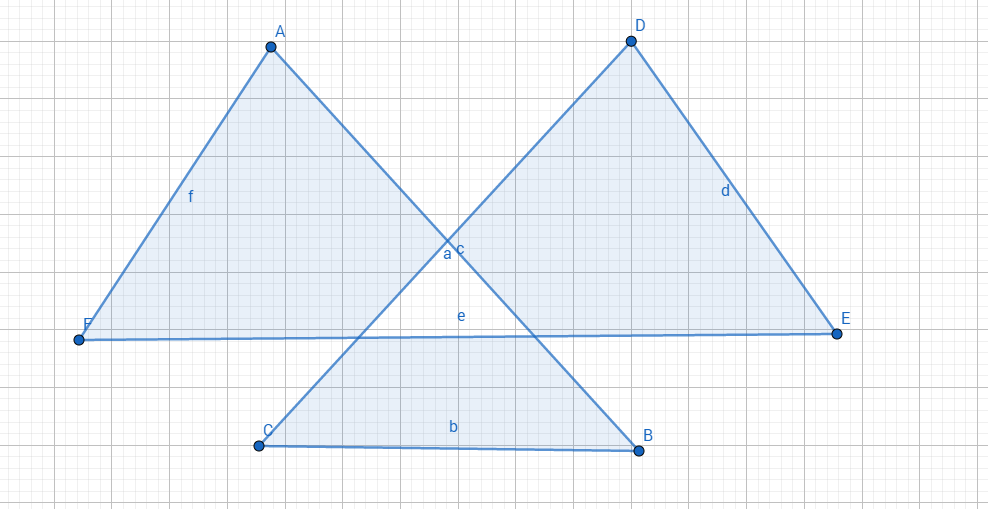
\includegraphics[width=0.5\textwidth]
    {figures/complex.png}
    \caption{复杂多边形的示例}
    \label{complex}
  \end{figure}

由于多边形的边界为一条闭合折线,易知对于每个多边形边界上的顶点,与其连接的边为偶数条。因此,射线的位置对相交次数的奇偶性不产生影响。

明确了划分规则后,我们可以采用逐层分离的方法将原多边形分割为简单多边形的组合。具体方法如下:

\begin{enumerate}
    \item 首先,对于多边形的边界,找出所有未被记录的交叉点,并将对应相交的边分别从交叉点处分割为两部分。
    \item 选择当前点集中x坐标最小的点,作为新多边形的起始点。
    \item 遍历当前点的所有连边,按极角序选择当前点到上一个点连线方向顺时针连接到的第一条边\footnote{对于第一个点从x轴负方向开始},将另一个端点加入当前多边形。
    \item 转到3 直至返回初始点。
    \item 记录当前多边形,并删除当前多边形对应的边和连边数小于2的顶点。
    \item 转到2 直至点集为空。
    \item 对于切割出的每个多边形,计算其内部到多边形外跨越的边数,判断其是否为孔洞。
\end{enumerate}

该算法的本质是记录所有未被顶点标记的交叉点,并重新计算原多边形的边界,判断多边形中每一条边具体所属的多边形边界曲线。
\section{消除多边形内部的孔洞}
通过在顶点上添加桥边和辅助节点,我们可以通过一次切割联通两个多边形孔洞,或是将一个多边形孔洞与外界相连。如图~\ref*{merge}所示,在添加额外的两个顶点和两条边后,两个多边形孔洞的边界将会合并为一个连续的环,而其代表的多边形区域不发生改变。由此,通过数次合并后,原有的带孔多边形将变为不含孔洞的凹多边形。
\subsection{预处理}
为确保多边形孔洞合并后点的顺序正确,边界不产生交叉,需要提前对多边形孔洞的顶点方向进行预处理。

我们令多边形外圈的点以逆时针顺序排列,内圈孔洞则以顺时针顺序排列。如此处理之后,两个多边形孔洞在合并时将保持正确的旋转方向,避免边界出现交叉。

\begin{figure}[htp]
    \centering
    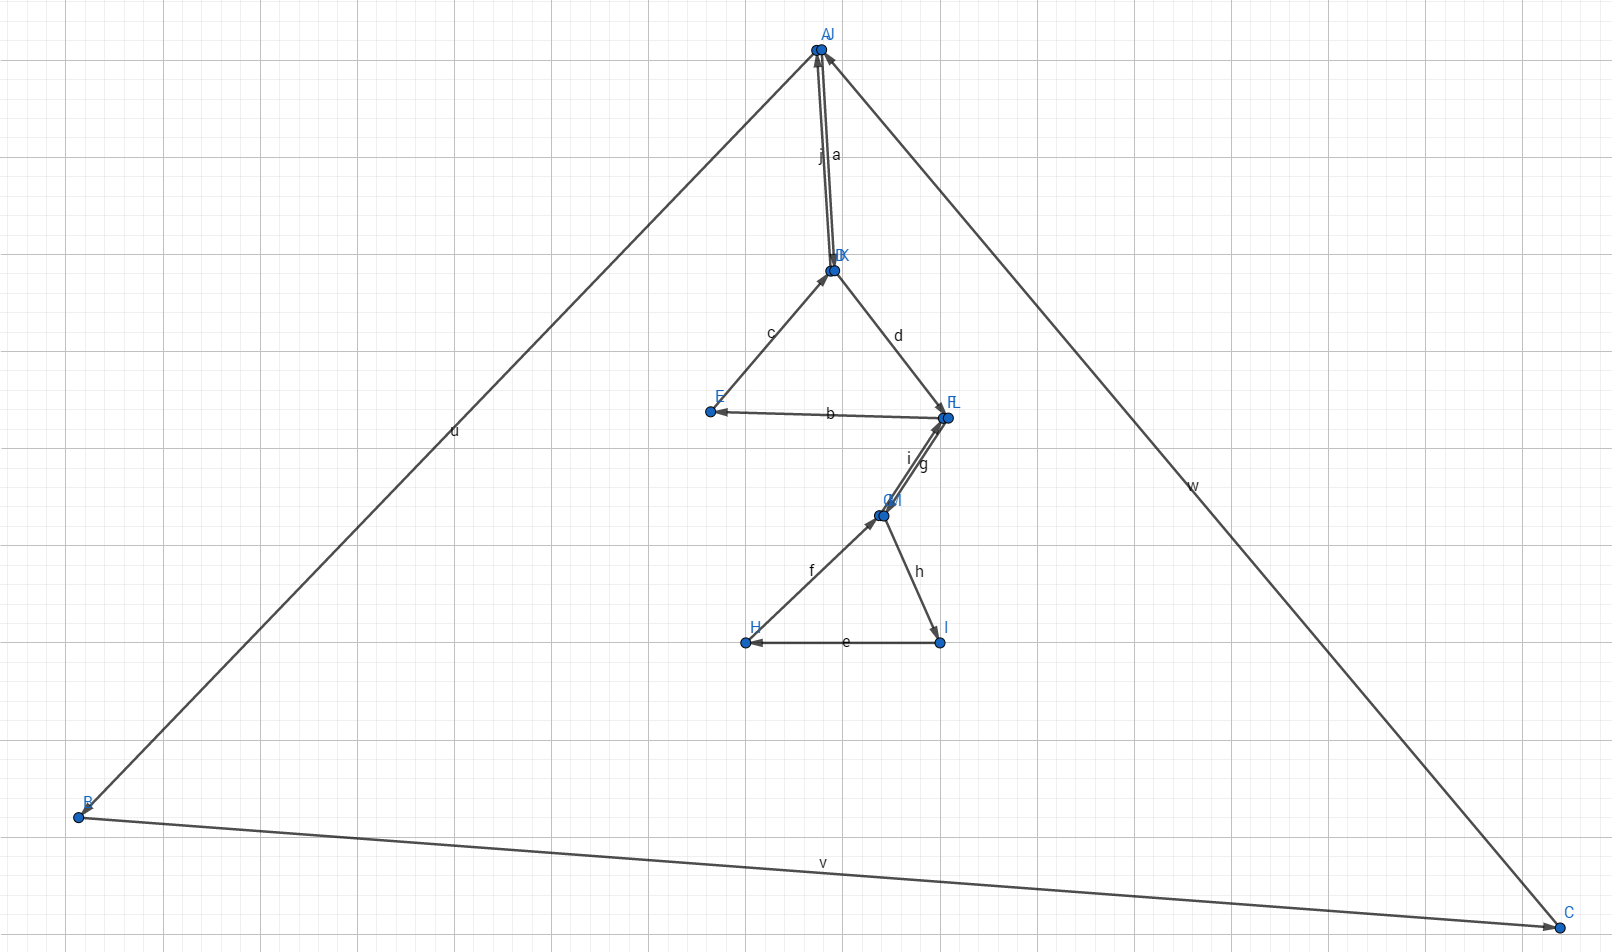
\includegraphics[width=0.5\textwidth]
    {figures/mergehole.png}
    \caption{正确处理多边形旋转顺序后的合并}
    \label{merge}
  \end{figure}

\subsection{朴素的合并方式}
将多边形上的所有点按照x坐标从小到大为第一关键字,y坐标从大到小为第二关键字排序。
按顺序遍历所有顶点,并记录当前已经遍历的所有节点所属的边界。
当新遍历到的顶点所属的边界与之前的边界未进行过合并时,选择之前遍历过的顶点之中与当前点距离最近的顶点,向其延伸一条射线,并于第一段相连的多边形边界处相连。以此线段作为切割线,合并相关联的两个边界。

遍历多边形上的所有节点后,多边形的每个孔洞都直接或间接的与多边形外边界相连,因此我们便可以消除多边形内部的孔洞。
\subsection{对上述算法的改良}
借助最小生成树的思路,我们可以最小化切割边的总长度。

枚举多边形中的每对分属两个不同多边形孔洞的点对,并判断其连线是否与其他边冲突,记录所有合法的切割边。

将切割边按长度从小到大排序,按顺序处理边。对于每条切割边,若切割边所连接的两部分多边形未被合并,且该边与已有的切割边之间不产生冲突,则沿此切割边将两侧的多边形边界合并为一体。当选择的切割边数目恰好与多边形孔洞数目相等时,所有的多边形边界均合并完成,原多边形的孔洞消除完成。

\subsection{采用分治法合并孔洞}
我们可以采用分治计算Delaunay triangulation算法中的思想,使用相似的方法完成对孔洞的合并。

首先将多边形孔洞的所有点按照x坐标从小到大为第一关键字,y坐标从大到小为第二关键字排序。接下来每次将待处理的点集分为左右两半,递归合并点集中的不同多边形片段。

当点集中的点不多于两个时,递归终止。若点集中的点分属不同多边形,则添加一条新的切割边连接两个顶点,将其加入候选集合。

接下来我们处理两个点集答案的合并。

从原多边形孔洞的边集中搜索,判断是否存在原有的连接两半点集的边。

若不存在这样的边,则使用分治计算Delaunay triangulation算法中的计算方式,找出所有合法的LR-edge,在候选集合中修正与之冲突的切割边,并额外添加一条最短的LR-edge至集合中。此处的合法LR-edge计算方式与分治计算Delaunay triangulation算法中的相似,但是寻找可行端点时需要排除连边时会与原多边形中已有的边产生冲突的顶点。

若存在连接两半点集的边,则将其直接加入集合,在候选集合中删除与之冲突的切割边,并寻找一条额外的切割边,连接原切割边所连接的集合。

由此思路,即可完成对所有孔洞的合并。接下来取孔洞中与边界距离最短的点对相连即可将多边形的孔洞消除。

%%%%%%%%%%%%%%%%%%%%%%%%%%%%%%%%%%%%%%%%%%%%%%%%%%%%%%%%%%%%%%%%%%%%%
\section{分割不含孔洞的凹多边形}


\subsection{确定多边形方向}
为了便于后续计算,我们规定多边形S的点依次逆时针排列。在计算时我们需要将初始的多边形端点标准化为按逆时针排序。
利用向量叉积的原理,我们可以计算出多边形的方向。
对于多边形的每条边,计算坐标原点到起点的向量,与边起点到终点的向量叉乘并除以2。将结果求和后该向量的模即为多边形面积,而向量z轴方向则代表了多边形的旋转方向。

\begin{equation}
\sum\limits_{i=0}^{n}{\frac{N_i\times (N_{(i+1)\bmod n}-N_i)}{2}}
\end{equation}

计算出初始多边形旋转方向后,即可根据需求调整端点的顺序以标准化多边形的方向。

\subsection{确认多边形凹凸性}
首先我们遍历多边形的所有内角,检测其是否为凸多边形。

若多边形为凸多边形,转至~\ref*{sec:对凸多边形进行三角化},直接生成其Delaunay三角划分;若多边形为凹多边形,则采用下面的算法将其分割为数个凸多边形。
\subsection{确定分割方案}
在这一步我们采用启发式搜索的方式进行分割。

我们定义合法的切割边\(( V_i,V_j) \)满足以下条件:

\begin{itemize}
    \item \(V_i,V_j\)属于同一个多边形
    \item 以\(V_i,V_j\)为端点的线段除端点外与多边形无共同点
    \item \(V_i,V_j\)两个顶点对应的多边形内角至少有一个大于180°
    \item \(0\le i<j\le n-1\)
\end{itemize}
对于原多边形S中的一条合法的切割边,我们采用如下方式来评估其价值:

\begin{itemize}
    \item 设按此方式切割后产生的两个多边形为

    \(S_1:\{ V_0,V_1,\cdots,V_{i-1},V_i,V_j,V_{j+1},\cdots,V_{n-1}\} \)

    \(S_2:\{ V_i,V_{i+1},\cdots,V_{j-1},V_j\}\)

    定义\(C(S_i)\)为多边形\(S_i\)的周长,\quad \(L(V_i,V_j)\)为点\(V_i,V_j\)之间的距离

    \item 定义切割边的基础评分为
    \begin{equation}
        \frac {\min(C(S_1),C(S_2))}{L(V_i,V_j)}
    \end{equation}
    \item 定义切割边的评分修正为
    \begin{equation}
        \frac {\min(\angle V_jV_iV_{i-1},\angle V_jV_iV_{i+1},\angle V_iV_jV_{j-1},\angle V_iV_jV_{j+1})}{90^\circ}
    \end{equation}

    若切割边两个端点对应的内角均>180°则评分修正额外*10

    \item 每条边的价值最终评估为基础评分*评分修正。
    
\end{itemize}

遍历多边形,对于每一个内角大于180°的顶点,采用此算法\upcite{金文华1999简单多边形可见点问题的快速求解算法}快速求出以该点为端点的所有合法切割边,计算其价值并加入记录。

\begin{figure}[htp]
    \centering
    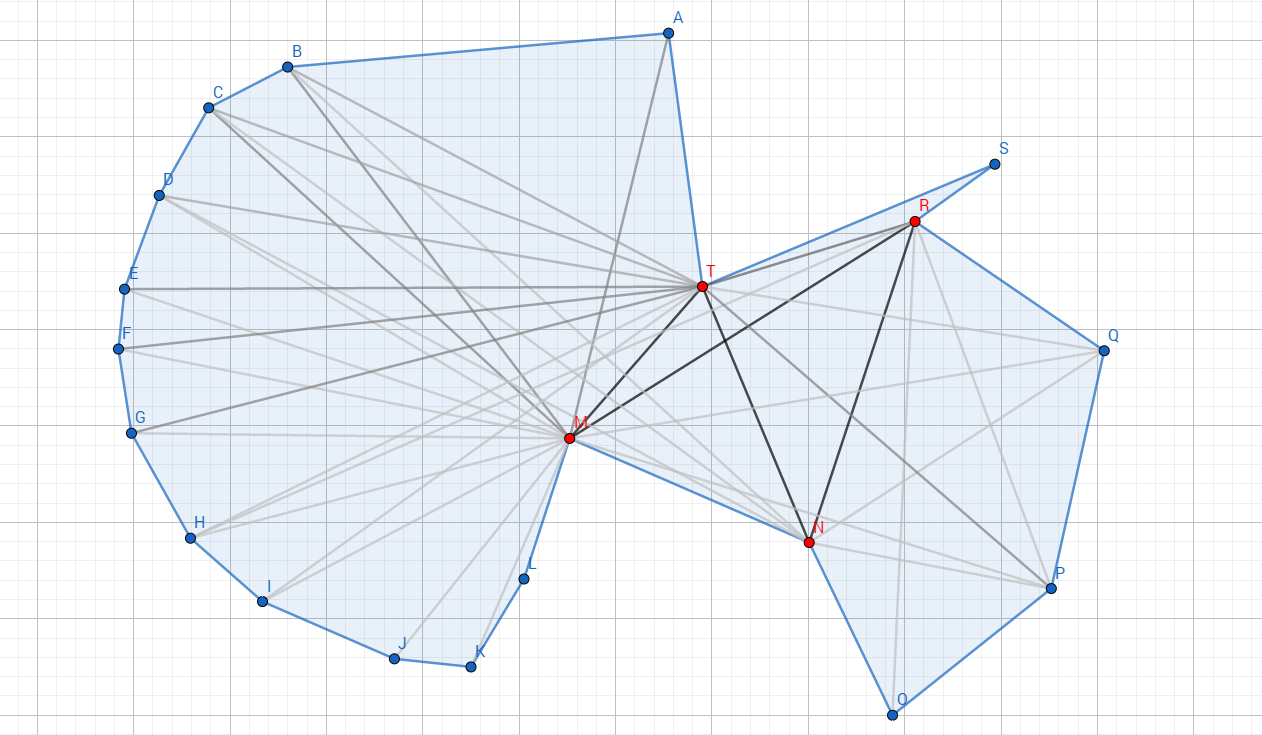
\includegraphics[width=0.5\textwidth]
    {figures/pass1.png}
    \caption{对候选边进行估价}
    \label{pass1}
\end{figure}

接下来对于所有合法的切割边,将其以价值从大到小排序,依次尝试加入分割列表。

当我们尝试将一条合法切割边加入分割方案时,在已经选定的分割方案中检查是否存在与当前切割边冲突的方案。若存在冲突则直接跳过该边。
具体来说,若两条切割边在非顶点的位置相交,则说明两种分割方案互相冲突,无法同时选用。此时我们选择价值相对较高者。

当我们计算得出了分割方案后,即可开始进行下一步的实际分割。

\subsection{对凹多边形进行分割}

确定了全部的可行分割方案后,我们可以开始划分凹多边形。

具体实现流程如下:
\begin{enumerate}
    \item 对分割方案\(V_i,V_j\)排序,以\(i\)为第一关键字递增,以\(j\)为第二关键字递减。
    \item 若栈顶元素\(V_{stk}\)满足\(stk<j\)则弹出栈顶元素直至\(stk\ge j\)。
    \item 若栈顶元素\(V_{stk}\)满足\(stk=j\)则将当前分割方案中的\(V_j\)指向的节点变更为\(V_stk\),并弹出栈顶元素。
    \item 选择接下来的分割方案,将\(V_i,V_j\)节点复制一份为\(V_{i}^{'},V_{j}^{'}\)。
    \item 在链表中连接\(V_{i-1},V_i^{'},V_j\)与\(V_{j-1},V_j^{'},V_i\)。
    \item 将\(V_j\)加入栈中。
\end{enumerate}

\begin{figure}[htbp]
    \centering
    \begin{minipage}{0.4\textwidth}
        \centering
        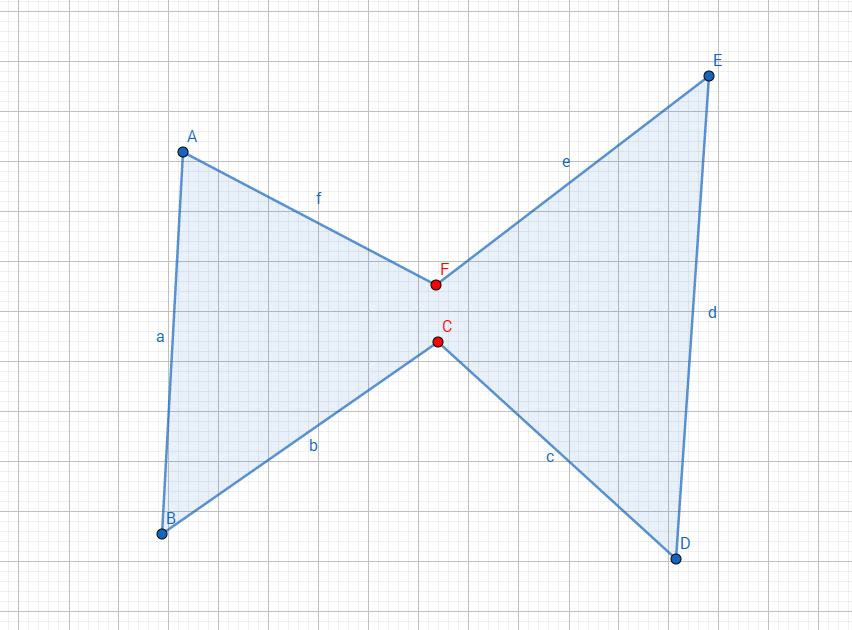
\includegraphics[width=0.95\textwidth]
        {figures/cut1.png}
        \caption{分割前的多边形}
    \end{minipage}
    \begin{minipage}{0.4\textwidth}
        \centering
        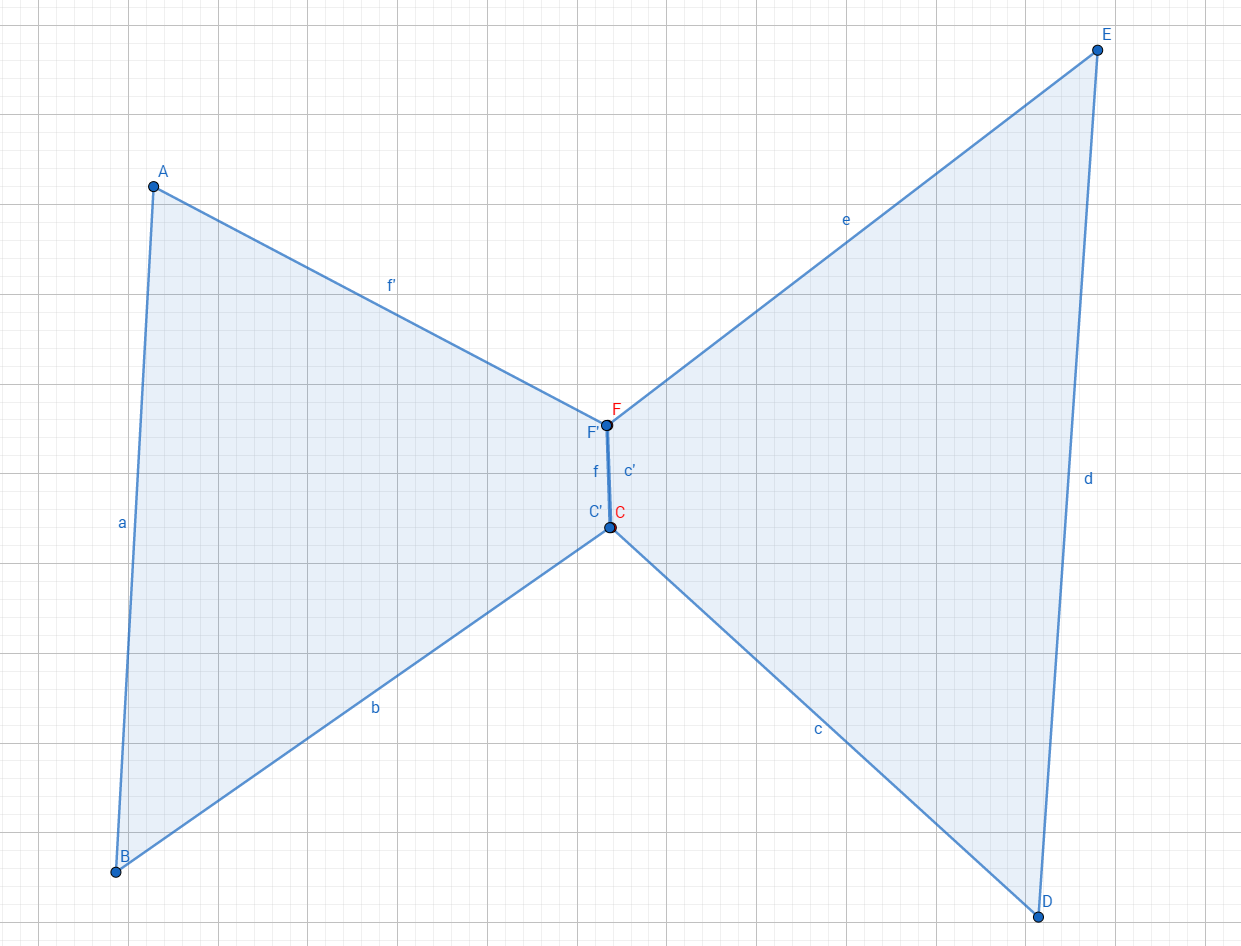
\includegraphics[width=0.95\textwidth]
        {figures/cut2.png}
        \caption{在待分割点的逆时针方向新增等位点}
    \end{minipage}
\end{figure}

以这种方案实现对多边形的分割时,可以巧妙的准确找到每个分割边所对应的顶点的真实位置。即使顶点被复制多次,初始指向顶点的指针指向了错误的多边形,也可以利用栈找到每个指针的正确位置。

完成上述流程后,原本的一个凹多边形将被分为数个部分,我们只需递归的对每个子多边形使用相同方式进行处理即可。

\begin{figure}[htp]
    \centering
    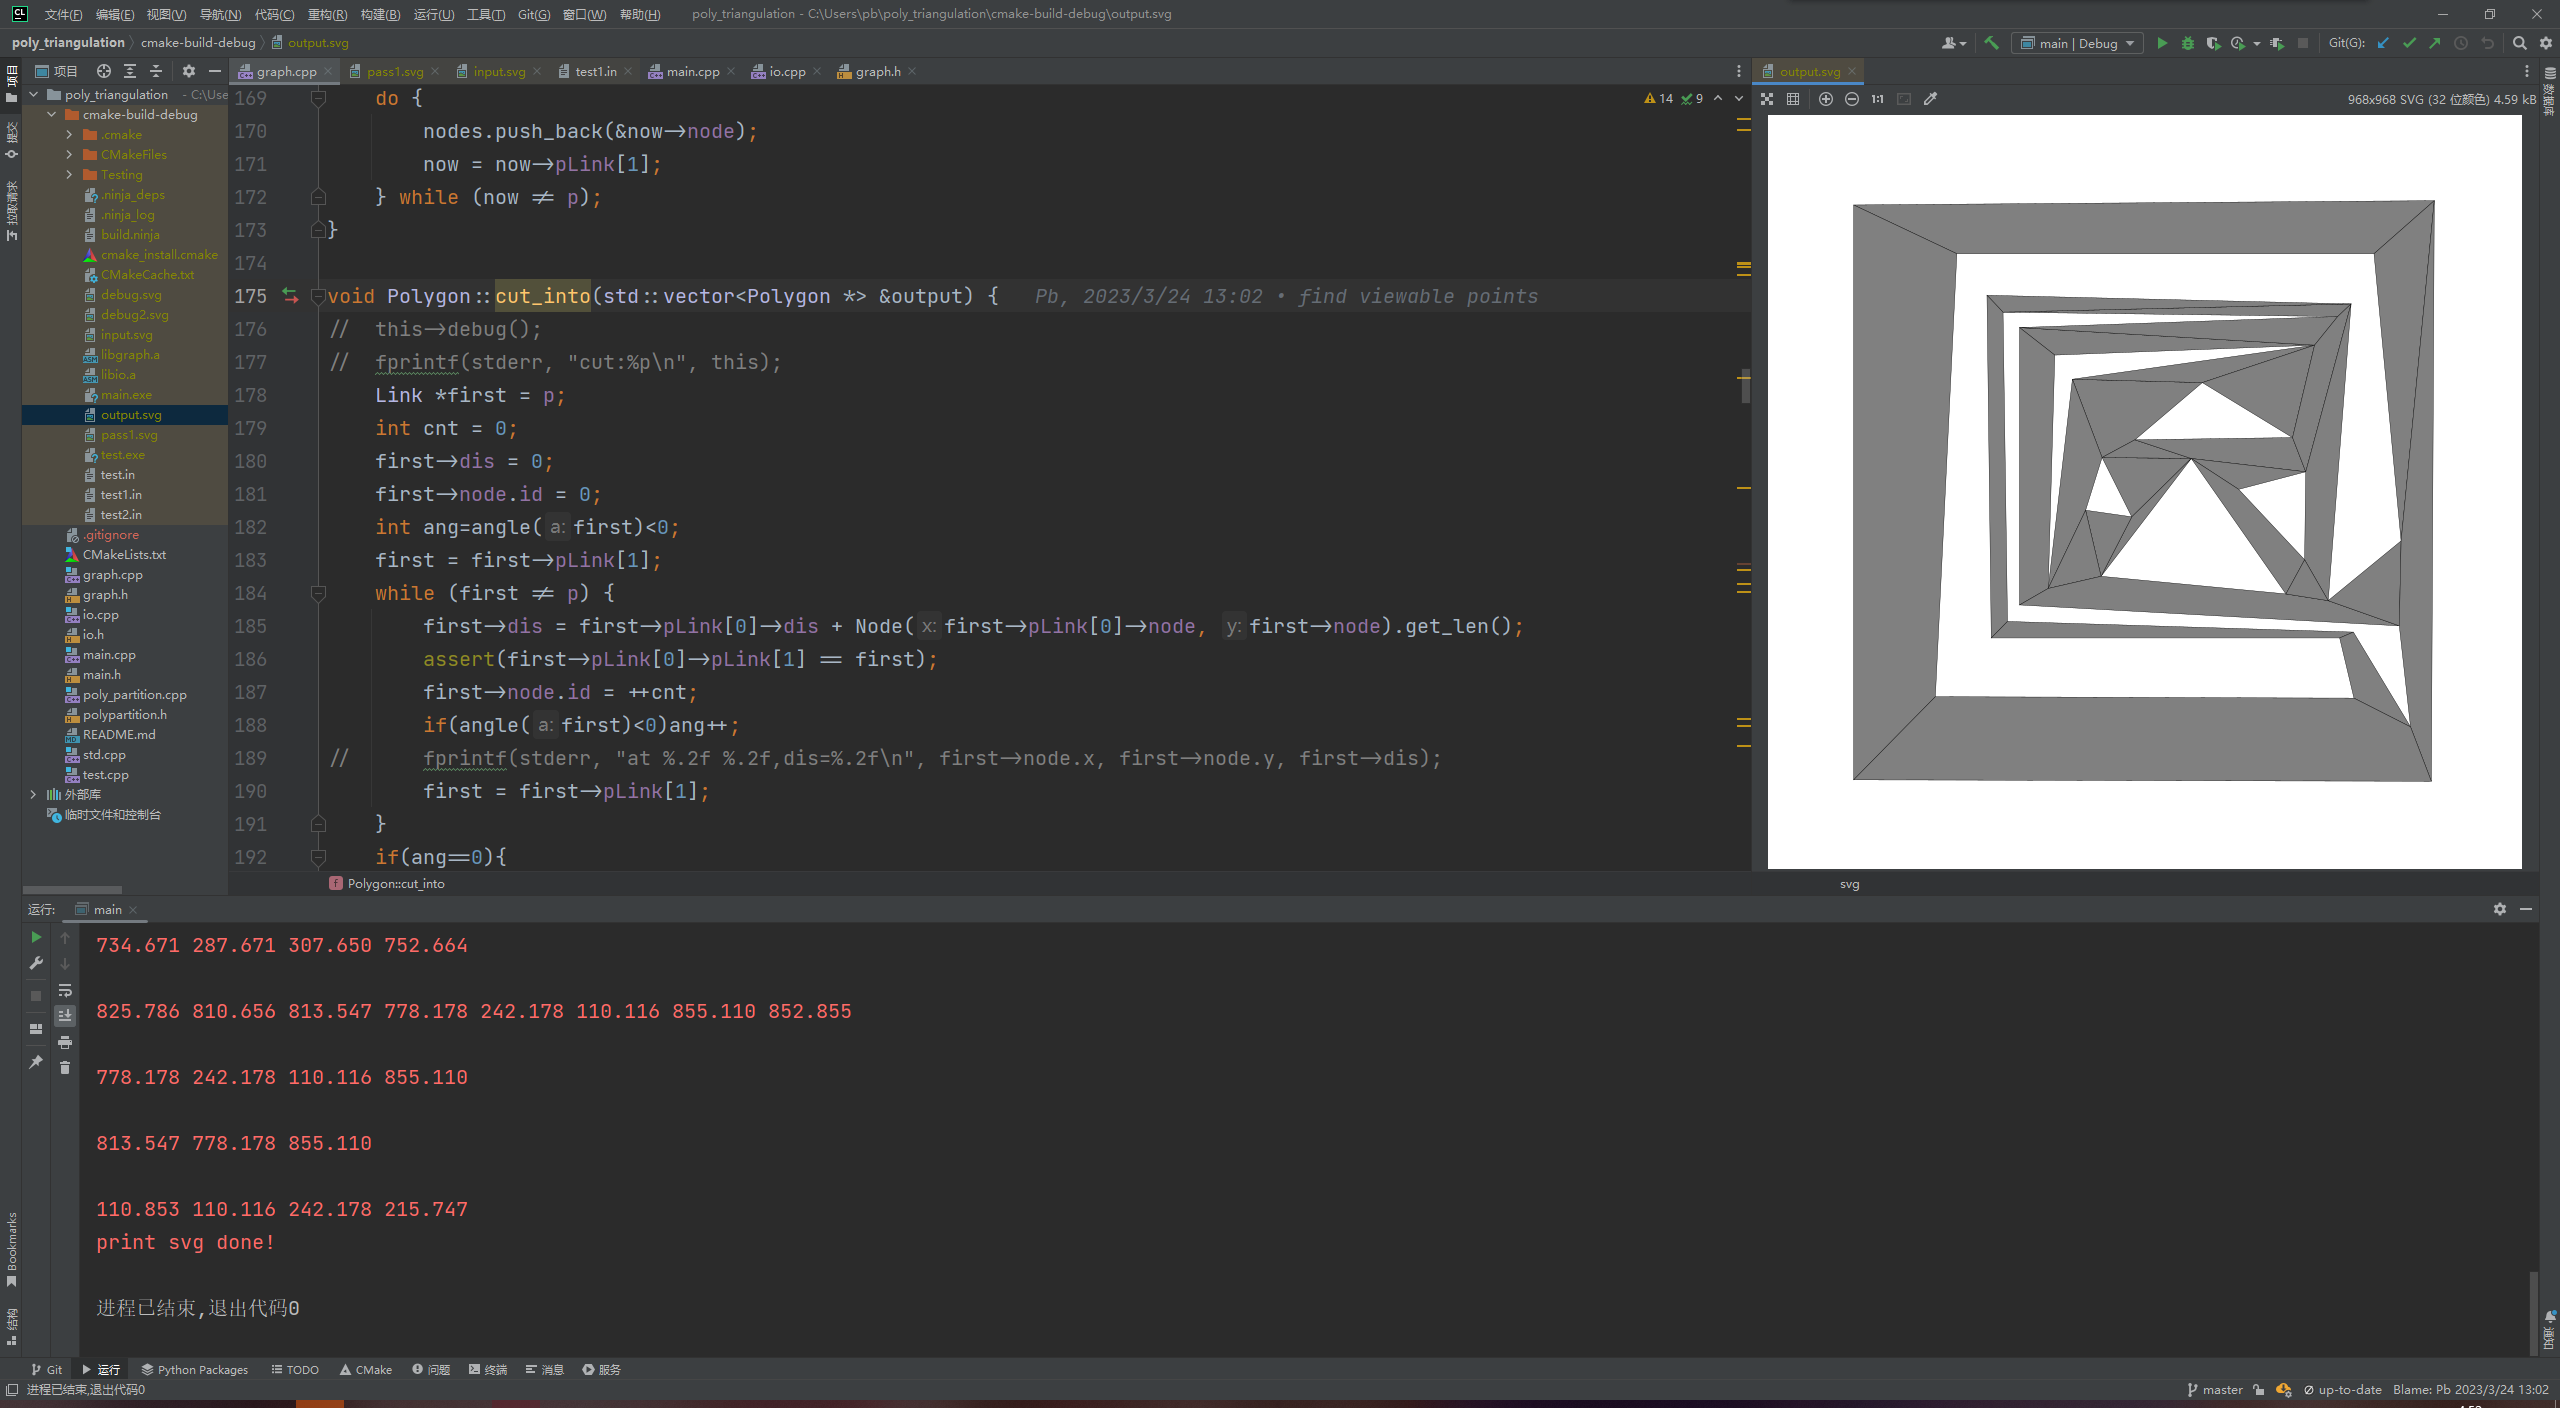
\includegraphics[width=0.9\textwidth]
    {figures/output.png}
    \caption{代码运行到此步的结果}
  \end{figure}

\subsection{一些其他的改进思路}
本算法可以较为有效的将凹多边形分割为数个凸多边形,但生成分割边时将会尽可能多的对原多边形进行分割,可能会在单个凹点处进行过多的切割,导致出现较小的锐角。对应图~\ref*{pass1}的情况,尽可能多的选择分割边时将会对一些评分较低不需要进行分割,但并未和已选边产生冲突的垃圾边也进行切割,导致产生大量的细长三角形。以下是一些改进本算法的思路。

\subsubsection{限制分割线数量}
在确定可行分割方案的过程中,默认采用了贪心算法,只要存在可行的分割方法就会加入结果中。因此可能会出现从一个凹顶点连线到凸多边形每个顶点进行分割的情况;而理想情况下本章算法的目标为用相对较少的线段将输入的凹多边形分割为数个凸多边形。因此,我们可以对分割线的数量进行限制。

在较为理想的情况下,每一条分割线可以消除1-2个凹点。也就是说,将一个凹多边形分割为数个凸多边形时,使用的分割线数目很可能少于凹顶点的数目。因此,我们可以限制每次选择分割方案的数目上限。

我们可以在算法的开始阶段记录当前多边形的凹顶点数目,并将其乘上一个修正量后作为分割线的最大数目。在依次检验分割方案是否与已选中部分冲突时,若已选中的分割线数目已经等于最大数目,则丢弃剩余的所有方案,只使用有限数量的分割线进行分割。由于被分割出的小多边形会用递归的方式再次经过本算法检验凹凸性并进行分割,算法的正确性不会受到影响。

正确的选择修正量可以在精确度与速度之中做出平衡。较大的修正量会产生更多的分割线,生成的小多边形将更不可能是需要重新执行本算法的凹多边形;而较小的修正量则能够获得较为优秀的划分结果,但会增加算法的运行时间。笔者认为,在实际计算中取0.5至1的修正量较为合适。

\subsubsection{禁止单个顶点进行多次切分}
在评估时,单个凹顶点可能有相似的数个较优秀候选切割边。这些切割边之间互不冲突,且评估价值相近。在筛选分割方案时,容易出现单个顶点选择数条同质切割边的情况。不仅会产生一些细长三角形,同时还影响算法效率。可以在切分时限制单个顶点最多被切分一次,跳过后续的相似切割边。
\subsubsection{动态调整启发函数}
在启发式函数中,采用的评估方案通过计算边长与切下的小多边形周长比值作为基础评分,以顶点凹凸性和最小角度数作为修正值。但在完成了一次切割后,后续的待选切割边两端的多边形周长将会发生变化,实际评估值将会改变,需要随时进行更新。考虑到实际评估值在分割过程中仅会下降不会上升,我们可以利用大根堆存储所有的切割方案,并在取新方案时对该方案进行更新并重新放入堆中,直到取出的方案已被更新过。

%%%%%%%%%%%%%%%%%%%%%%%%%%%%%%%%%%%%%%%%%%%%%%%%%%%%%%%%
\section{对凸多边形进行三角化}\label{sec:对凸多边形进行三角化}

最终的凸多边形\footnote{每个内角均小于\(180°\)的多边形}是平面多边形中最简单最易处理的一类。

我们在实现了对凸多边形的三角化后即完成了整个算法。

\subsection{朴素的划分方案}

由于凸多边形的性质,多边形任意两个顶点之间连边均在多边形内部。因此最简单的划分方案即为 对于\(i\in [2,n-2]\),沿边\(S_0,S_i\)进行一次分割,即可产生总共n-2个三角形。该方案最为简便,且产生的三角形均有一个共同顶点,但产生的三角形形状均为细长型,相对形态较劣。
\begin{figure}[htp]
    \centering
    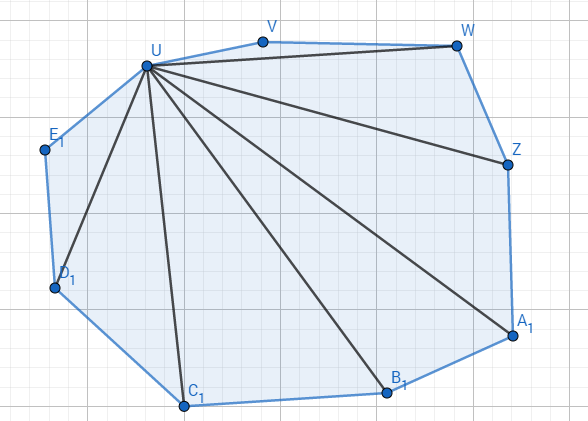
\includegraphics[width=0.5\textwidth]
    {figures/凸多边形1.png}
    \caption{最简单的一种三角划分策略}
  \end{figure}

\subsection{改进的朴素划分}

由于对凸多边形分割后产生的两个多边形仍为凸多边形,我们可以采用分治法来一定程度的优化上述方案。
一种可行的方案如下:
\begin{itemize}
    \item 若当前多边形为三角形则结束算法;
    \item 随机选择两个不相邻的顶点连边,将当前多边形分割为两部分;
    \item 对分割出的两个子多边形调用本算法进行分割,并将分割的结果加入答案。
\end{itemize}

沿着这个方向,该方案仍然有一定的优化空间。我们若倾向于每次尽可能的将多边形分割为面积相似,形状接近圆形的两个部分,分割的最终结果将会更加优秀。但是该方案代价相对较大,且最终产生的结果相比于随机法并没有显著的提升。

\begin{figure}[htp]
    \centering
    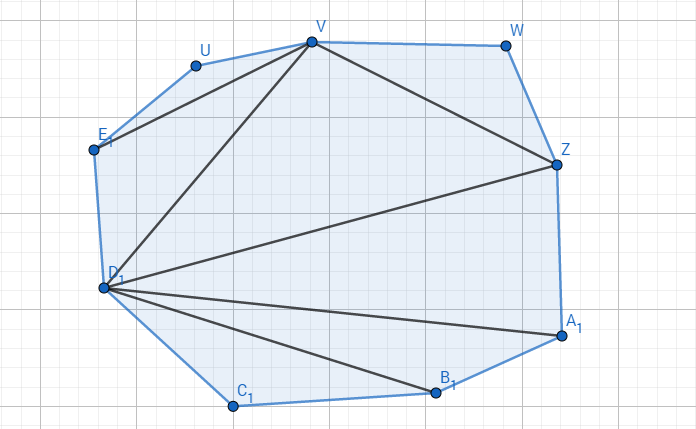
\includegraphics[width=0.5\textwidth]
    {figures/random.png}
    \caption{经过随机化优化后的分割结果}
  \end{figure}

\subsection{完美三角剖分}
Delaunay triangulation(简称DT)是一种三角剖分方式,其结果满足以下性质:
\begin{itemize}
    \item 对于三角剖分中产生的每一个三角形,其外接圆中不包含点集V中的其他点。
    \item 若对点集的三角剖分结果中每一个三角形的最小角升序排列,则DT所得到的数值比其他三角剖分的数值大。
    \item 若点集中任意四点均不共圆,则产生的三角剖分唯一。
\end{itemize}

\begin{figure}[htbp]
    \centering
    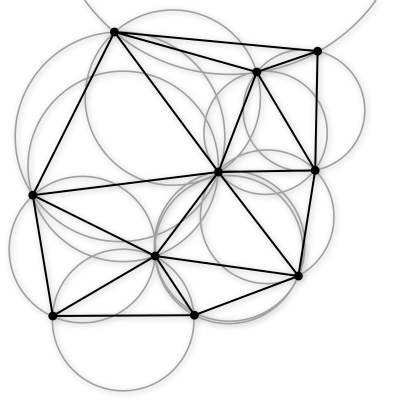
\includegraphics[width=0.4\textwidth]
    {figures/triangulation-1.png}
    \caption{Delaunay triangulation的分割结果}
\end{figure}

若进行三角剖分的点集中存在四点共圆,虽然计算其Delaunay triangulation时得到的结果不唯一,但仍不破坏其余性质。由于最小角最大的特性,DT可以产生理论最优的划分。而根据三角剖分的性质,对凸多边形顶点点集进行三角剖分所得到的三角形集合即为待求的三角化结果。

一种利用分治思想在\(O(n\log n)\)复杂度内计算点集的Delaunay triangulation方法如下:

首先将给定点集按照 x 坐标升序排列,如图~\ref*{DT1}所示。

\begin{figure}[htbp]
    \centering
    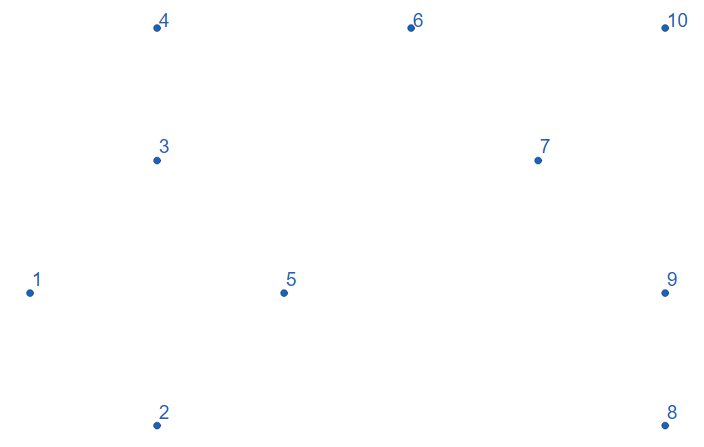
\includegraphics[width=0.5\textwidth]
    {figures/DT1.png}
    \caption{排好序的大小为10的点集}
    \label{DT1}
\end{figure}
\newpage
一旦点集有序,我们就可以不断地将其平分成两个部分,直到子点集大小不超过 3。然后这些子点集可以立刻剖分为一个三角形或线段。

\begin{figure}[htbp]
    \centering
    \begin{minipage}{0.4\textwidth}
        \centering
        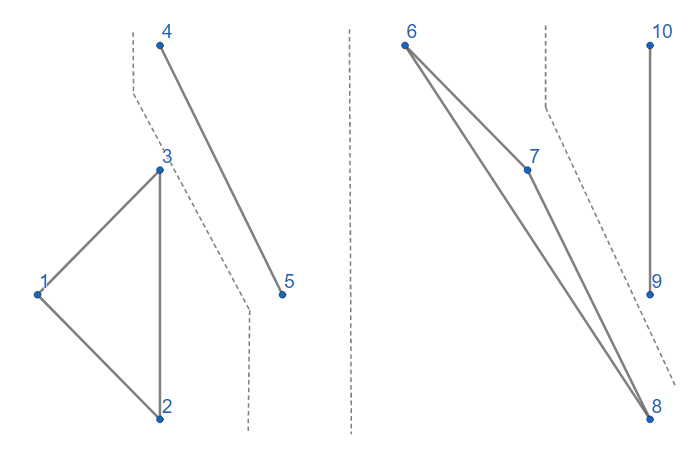
\includegraphics[width=\textwidth]
        {figures/DT2.png}
        \caption{分治为包含2或3个点的点集}
    \end{minipage}
    \begin{minipage}{0.4\textwidth}
        \centering
        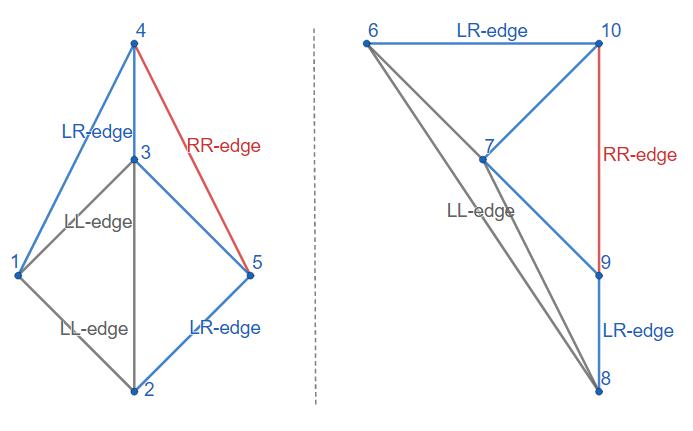
\includegraphics[width=\textwidth]
        {figures/DT3.png}
        \caption{三种不同的边}
        \label{DT3}
    \end{minipage}
\end{figure}

在分治回溯的过程中,已经剖分好的左右子点集可以依次合并。合并后的剖分包含 LL-edge(左侧子点集的边)。RR-edge(右侧子点集的边),LR-edge(连接左右剖分产生的新的边),如图~\ref*{DT3} LL-edge(灰色),RR-edge(红色),LR-edge(蓝色)。对于合并后的剖分,为了维持 DT 性质,我们可能需要删除部分 LL-edge 和 RR-edge,但我们在合并时不会增加 LL-edge 和 RR-edge。


合并左右两个剖分的第一步是插入 base LR-edge,base LR-edge 是最底部的不与任何LL-edge 及 RR-edge 相交的 LR-edge。


然后,我们需要确定下一条紧接在base LR-edge 之上的 LR-edge。比如对于右侧点集,下一条 LR-edge 的可能端点(右端点)为与 base LR-edge 右端点相连的 RR-edge 的另一端点(6, 7, 9 号点),左端点即为 2 号点。
\begin{figure}[htbp]
    \centering
    \begin{minipage}{0.4\textwidth}
        \centering
        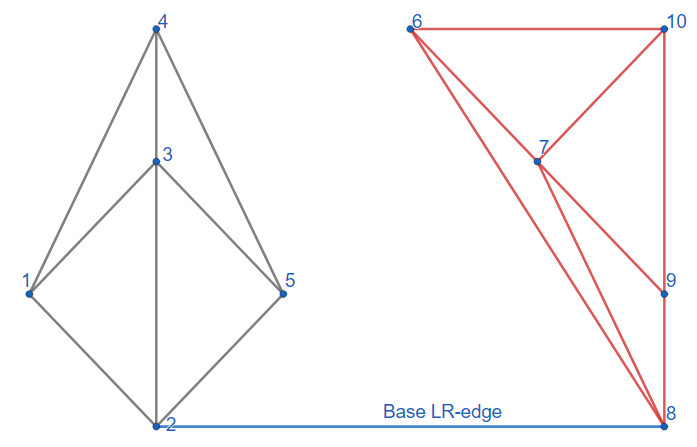
\includegraphics[width=\textwidth]
        {figures/DT4.png}
        \caption{合并左右剖分}
    \end{minipage}
    \begin{minipage}{0.4\textwidth}
        \centering
        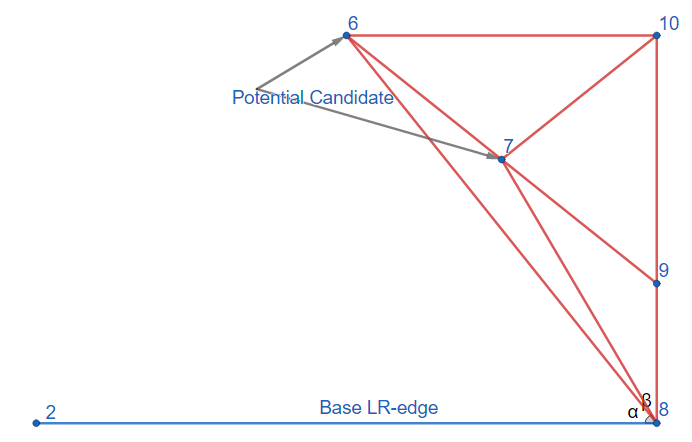
\includegraphics[width=\textwidth]
        {figures/DT5.png}
        \caption{下一条LR-edge的可能位置}
    \end{minipage}
\end{figure}

对于可能的端点,我们需要按以下两个标准检验:

\begin{enumerate}
    \item 其对应 RR-edge 与 base LR-edge 的夹角小于 180 度。即,新选择的端点在当前base LR-edge的“上方”。
    \item base LR-edge 两端点和这个可能点三点构成的圆内不包含任何其它可能点。
\end{enumerate}

如图~\ref*{DT6},6 号可能点所对应的绿色圆包含了 9 号可能点,而 7 号可能点对应的紫色圆则不包含任何其它可能点,故 7 号点为下一条 LR-edge 的右端点。

对于左侧点集,我们做镜像处理即可。

当左右点集都不再含有符合标准的可能点时,合并即完成。当一个可能点符合标准,一条 LR-edge 就需要被添加,对于与需要添加的 LR-edge 相交的 LL-edge 和 RR-edge,将其删除。

当左右点集均存在可能点时,判断左边点所对应圆是否包含右边点,若包含则不符合;对于右边点也是同样的判断。在未出现四点共圆的情况下每次只会有一个可能点符合标准,否则任选其一即可。

\begin{figure}[htbp]
    \centering
    \begin{minipage}{0.32\textwidth}
        \centering
        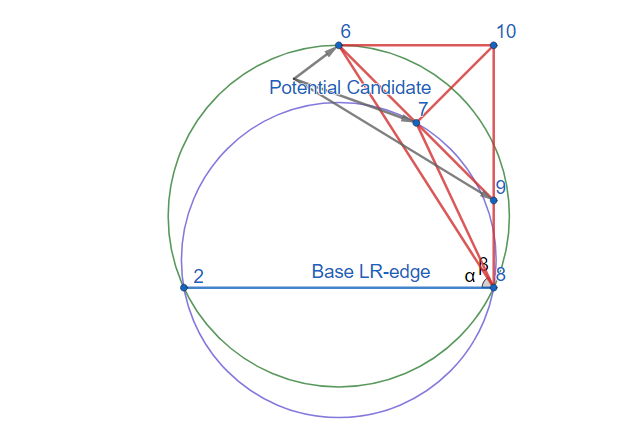
\includegraphics[width=\textwidth]
        {figures/DT6.png}
        \caption{检验可能点}
        \label{DT6}
    \end{minipage}
    \begin{minipage}{0.32\textwidth}
        \centering
        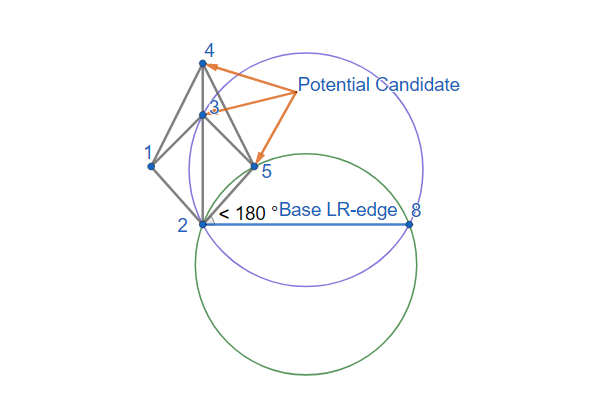
\includegraphics[width=\textwidth]
        {figures/DT7.png}
        \caption{镜像处理另一半点集}
    \end{minipage}
    \begin{minipage}{0.32\textwidth}
        \centering
        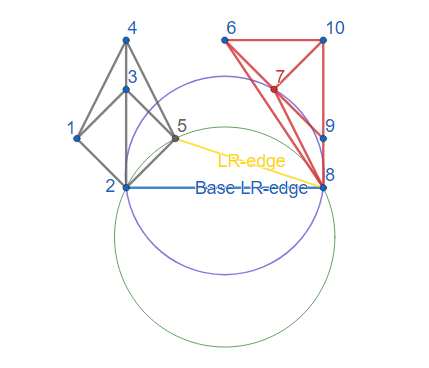
\includegraphics[width=\textwidth]
        {figures/DT8.png}
        \caption{下一条LR-edge}
    \end{minipage}
\end{figure}



重复以上步骤即可完成Delaunay triangulation的构建。

由此我们完成了对任意多边形的三角化。
% \section{公式的使用}
% 在文中引用公式可以这么写:$a^2+b^2=c^2$这是勾股定理,他还可以表示为$c=\sqrt{a^2+b^2}$,还可以让公式单独一段并且加上编号。注意,公式前请不要空行。
% \begin{equation}
% \sin^2{\theta}+\cos^2{\theta}=1 \label{eq:pingfanghe}
% \end{equation}

% 还可以通过添加标签在正文中引用公式,如式\eqref{eq:pingfanghe}。

% 我们还可以轻松打出一个漂亮的矩阵:
% \begin{equation}
%   \mathbf{A}=
%   \left[\begin{matrix}
%     1&2&3&4\\
%     11&22&33&44\\
%   \end{matrix}\right] \times
%   \left[\begin{matrix}
%     22&24\\
%     32&34\\
%     42&44\\
%     52&54\\
%   \end{matrix}\right]
% \end{equation}

% 或者多行对齐的公式:
% \begin{equation}
%   \begin{aligned}
%     f_1(x)&=(x+y)^2\\
%           &=x^2+2xy+y^2
%   \end{aligned}
% \end{equation}


% \section{插图的使用}

% \LaTeX 环境下可以使用常见的图片格式:JPEG、PNG、PDF、EPS等。当然也可以使用\LaTeX 直接绘制矢量图形,可以参考pgf/tikz等包中的相关内容。需要注意的是,无论采用什么方式绘制图形,首先考虑的是图片的清晰程度以及图片的可理解性,过于不清晰的图片将可能会浪费很多时间。

% 图示例如下:

% \begin{figure}[!htb]
%   \centering
%   \includegraphics[width=0.3\textwidth]
%   {figures/whulogo.png}\\
%   \caption{插图示例}
%   \label{fig:whu}
% \end{figure}

% \verb|[htbp]|选项分别是此处、页顶、页底、独立一页。\verb|[width=\textwidth]|让图片占满整行,或\verb|[width=2cm]|直接设置宽度。可以随时在文中进行引用,如图~\ref{fig:whu},建议缩放时保持图像的宽高比不变。

% \section{表格的使用}

% 表格的输入可能会比较麻烦,可以使用在线的工具,如~\href{https://www.tablesgenerator.com/}{Tables Generator}~能便捷的创建表格,也可以使用离线的工具,如~\href{https://ctan.org/pkg/excel2latex}{Excel2LaTeX}~支持从Excel表格转换成\LaTeX{}表格。\href{https://en.wikibooks.org/wiki/LaTeX/Tables}{LaTeX/Tables}~上及~\href{https://www.tug.org/pracjourn/2007-1/mori/mori.pdf}{Tables in LaTeX}~也有更多的示例能够参考。

% \subsection{普通表格}
% 下面是一些普通表格的示例:

% \begin{table}[ht]
%   \centering
%   \caption{简单表格}
%   \label{tab:1}
%   \begin{tabular}{|l|c|r|}
%     \hline
%     我是& 一只 & 普通\\
%     \hline
%     的& 表格& 呀\\
%     \hline
%   \end{tabular}
% \end{table}

% \begin{table}[ht]
%   \centering
%   \caption{一般三线表}
%   \label{tab:2}
%   \begin{tabular}{ccc}
%     \hline
%     姓名& 学号& 性别\\
%     \hline
%     张三& 001& 男\\
%     李四& 002& 女\\
%     \hline
%   \end{tabular}
% \end{table}

% \subsection{跨页表格}
% 跨页表格常用于附录(把正文懒得放下的实验数据统统放在附录的表中),以下是一个跨页表格的示例:

% {\centering
%   \begin{longtable}{ccccccccc}
%   \caption{跨页表格示例} \\
%   \toprule
%   1     & 0 & 5  & 1  & 2  & 3  & 4  &  5 & 6 \\
%   \midrule
%   \endfirsthead

%   \multicolumn{1}{l}{接上一页} \\
%   \toprule
%   1     & 0 & 5  & 1  & 2  & 3  & 4  &  5 & 6 \\
%   \midrule
%   \endhead

%   \bottomrule
%   \hline \\
%   \multicolumn{9}{r}{{转下一页}} \\
%   \endfoot

%   \bottomrule
%   \endlastfoot    

%   1     & 0 & 5  & 1  & 2  & 3  & 4  &  5 & 6 \\
%   1     & 0 & 5  & 1  & 2  & 3  & 4  &  5 & 6 \\
%   1     & 0 & 5  & 1  & 2  & 3  & 4  &  5 & 6 \\
%   1     & 0 & 5  & 1  & 2  & 3  & 4  &  5 & 6 \\
%   1     & 0 & 5  & 1  & 2  & 3  & 4  &  5 & 6 \\
%   1     & 0 & 5  & 1  & 2  & 3  & 4  &  5 & 6 \\
%   1     & 0 & 5  & 1  & 2  & 3  & 4  &  5 & 6 \\
%   1     & 0 & 5  & 1  & 2  & 3  & 4  &  5 & 6 \\
%   1     & 0 & 5  & 1  & 2  & 3  & 4  &  5 & 6 \\
%   1     & 0 & 5  & 1  & 2  & 3  & 4  &  5 & 6 \\
%   1     & 0 & 5  & 1  & 2  & 3  & 4  &  5 & 6 \\
%   1     & 0 & 5  & 1  & 2  & 3  & 4  &  5 & 6 \\

%   \end{longtable}
% }

% \subsection{统计表格}
% 要创建占满整个文字宽度的表格需要使用到tabularx,如不需要,使用tabular就行。引用表格与其它引用一样,只需要:表~\ref{tab:3},统计表格一般是三线表形式。

% \begin{table}[ht]
%   \centering
%   \caption{统计数据表格}
%   \label{tab:3}
%   \begin{tabularx}{\textwidth}{CCCC}
%     \toprule
%     序号&年龄&身高&体重\\
%     \midrule
%     1&14&156&42\\
%     2&16&158&45\\
%     3&14&162&48\\
%     4&15&163&50\\
%     \cmidrule{2-4} %添加2-4列的中线
%     平均&15&159.75&46.25\\
%     \bottomrule
%   \end{tabularx}
% \end{table}

% \section{列表的使用}
% 下面演示了创建有序及无序列表,如需其它样式,\href{https://www.latex-tutorial.com/tutorials/lists/}{LaTeX Lists}~上有更多的示例。

% \subsection{有序列表}
% 这是一个计数的列表
%   \begin{enumerate}
%       \item 第一项
%           \begin{enumerate}
%               \item 第一项中的第一项
%               \item 第一项中的第二项
%           \end{enumerate}
%       \item 第二项
%     \begin{enumerate}[label=(\roman*)]
%       \item 第一项中的第一项
%       \item 第一项中的第二项
%     \end{enumerate}
%       \item 第三项
%   \end{enumerate}

% \subsection{不计数列表}
%   这是一个不计数的列表
%   \begin{itemize}
%       \item 第一项
%       \begin{itemize}
%           \item 第一项中的第一项
%           \item 第一项中的第二项
%       \end{itemize}
%       \item 第二项
%       \item 第三项
%   \end{itemize}

% \section{定理的使用}
% \begin{theorem}
%   设向量$\boldsymbol a\neq\boldsymbol 0$,那么向量$\boldsymbol b//\boldsymbol a$的充分必要条件是:存在唯一的实数$\lambda$,使$\boldsymbol b=\lambda \boldsymbol a$。
% \end{theorem}
% \begin{definition}
%   这是一条定义。
% \end{definition}
% \begin{lemma}
%   这是一条引理。
% \end{lemma}
% \begin{corollary}
%   对数轴上任意一点$P$,轴上有向线段$\vec {OP}$都可唯一地表示为点$P$的坐标与轴上单位向量$\boldsymbol e_u$的乘积:$\vec {OP}=u \boldsymbol e_u$。
% \end{corollary}
% \begin{proposition}
%   这是一条性质。
% \end{proposition}
% \begin{example}
%   这是一条例。
% \end{example}
% \begin{remark}
%   这是一条注。
% \end{remark}